\chapter{Concetti e categorie}\index{categorie mentali}
La costruzione del sapere e della conoscenza è il risultato di un’attività fondamentale effettuata dagli esseri umani, ovvero la ``categorizzazione'', grazie alla quale l’unicità di ciascuna esperienza viene compresa e inserita nell’insieme più ampio delle categorie apprese e condivise. Nel momento in cui cogliamo delle somiglianze e delle differenze nella varietà infinita delle cose che ci circondano e raggruppiamo in classi o categorie le entità del mondo esterno compiamo un’operazione di grosso rilievo filosofico. La capacità di categorizzare, di percepire la similarità nelle diversità, di suddividere il continuo dell’esperienza in unità discrete è una delle abilità cognitive più importanti dell’uomo, e il linguaggio è in grado di riflettere queste abilità di categorizzazione.

Linguaggio, pensiero e realtà sono strettamente connessi nei processi di categorizzazione. A tale proposito, il primo a formalizzare il concetto fu Aristotele\index{Aristotele} con la cosiddetta \emph{concezione classica}, il cui presupposto è che le categorie sono definite in termini di congiunzione di caratteristiche necessarie e sufficienti.

Aristotele pone le basi per distinguere le \emph{proprietà necessarie e sufficienti} che definiscono una categoria. Una volta stabilita una categoria, l’universo risulta suddiviso in due insiemi di entità: quelle che sono membri della categoria e quelli che non lo sono. Le categorie sono cioè discrete, con confini netti e ben definiti, in modo che si possa stabilire con precisione cosa vi rientra e cosa no. Non ci sono entità ambigue, dunque non si può dire che vi siano entità che ``in qualche modo'' vi appartengono. Le categorie sono uniformi, organizzate gerarchicamente e le proprietà hanno tutte la stessa importanza. Il principio dominante in questo tipo di concezione è il principio dell’astrazione, per cui le categorie vengono costruite a partire dall’astrazione di tratti comuni delle cose del mondo. Inoltre le categorie sono costruite arbitrariamente, nel senso che non c’è nulla nel mondo che determini in che modo dobbiamo procedere nella categorizzazione. Ci troviamo di fronte alla realtà di un continuo diffuso e il nostro modo di categorizzarlo è un puro artificio della nostra cultura e della nostra lingua.

Tuttavia, a partire dalle riflessioni di Ludwig Wittgenstein\index{Wittgenstein, Ludwig}\footnote{Ludwig Josef Johann Wittgenstein (Vienna, 26 aprile 1889 – Cambridge, 29 aprile 1951) è stato un filosofo, ingegnere e logico austriaco, autore in particolare di contributi di capitale importanza alla fondazione della logica e alla filosofia del linguaggio.} (1953) a proposito del concetto di gioco e della nozione di \emph{somiglianza di famiglia}\index{somiglianza di famiglia} per descrivere le proprietà dei giochi (figura \ref{fig:famiglia}, ciò che caratterizza un concetto non sono tanto delle proprietà univoche e definibili una volta per tutte, ma, per l’appunto, delle somiglianze di famiglia, ossia delle proprietà che non sono sempre e tutte presenti in ogni esemplare della categoria che vogliamo definire, ma si distribuiscono in vario modo all’interno della categoria), le categorie non possono essere definite da un insieme chiuso di proprietà necessarie e sufficienti, ma hanno confini vaghi e sfumati e i loro membri sono disposti lungo un continuo alle cui estremità troviamo delle entità di cui possiamo dire con certezza cosa sono e cosa no (per esempio, una mela è un frutto e una patata non lo è). In tal senso, un aiuto alla formalizzazione delle categorie viene dalla teoria degli insiemi fuzzy (\S \ref{fuzzy-set}, pagina \pageref{fuzzy-set}).

\begin{figure}[hbt]
  \centering
  \includegraphics[width=\textwidth]{img/prototype-theory.png}
  \caption{Esempio di somiglianza di famiglia per descrivere le proprietà dei giochi}
  \label{fig:famiglia}
\end{figure}

\section{Categorie di parentela}
Floyd Lonsbury\index{Lonsbury, Floyd}, un antropologo cognitivo, nel 1964, pubblicò i suoi studi sul sistema di parentela delle tribù parlanti la lingua Fox tra gli indiani nativi americani. Le loro regole per nominare i parenti mostrano come le categorie possono essere definite da un \emph{elemento centrale} più alcune \emph{regole generative}.

Ad esempio, Lonsbury nota che la parola che indica il fratello della madre (zio) è \emph{nehcihsähA}, che è la l'elemento centrale. Attraverso una regola generativa la stessa parola si applica anche al figlio del figlio della madre della madre (cugino), al figlio del figlio del padre della madre della madre (figlio del prozio) e via dicendo. Nella tribù, ovviamente, si può distinguere gli zii dai prozii dai cugini, ma questi fanno tutti parte della stessa categoria di parentela, e quindi chiamati nello stesso modo. Queste categorie sono strutturate in modo da avere un membro focale e un piccolo insieme di regole generative che consentono di estendere ogni categoria a membri non focali.

\section{Categorie dei colori}
Il lavoro di Brent Berlin\index{Berlin, Brent} e Paul Kay\index{Kay, Paul} del 1969 mette esplicitamente in discussione la concezione per cui le categorie del colore sarebbero in definitiva le categorie arbitrarie e che non c’è nulla che ci obblighi a classificare i colori in un modo anziché in un altro. Berlin e Key prendono in esame 98 lingue (di cui 20 in dettaglio) e osservano che in ognuna di esse ci sono al massimo undici categorie codificate di colori fondamentali (rosso, verde, blu, giallo, nero, bianco, grigio, arancione, porpora, marrone, rosa), anche se non è detto che le lingue le codifichino tutte e undici. In generale, pur osservando una notevole variabilità individuale riguardo ai confini delle categorie dei colori, i soggetti esaminati appartenenti a comunità linguistiche differenti si mostrano quasi sempre d’accordo nel decidere quale sia il miglior esempio di una determinata categoria di colore. A partire dall’osservazione di un accordo più o meno universale riguardo ai membri centrali delle categorie, Berlin e Kay sono arrivati alla conclusione che le undici categorie di colori fondamentali sono degli \emph{universali percettivi}\index{universale percettivo}.

All'interno di una realtà continua (lo spettro dei colori) esistono quindi dei \emph{punti focali}\index{punto focale}, percettivamente più salienti di altri. La maggiore salienza dei punti focali non è dimostrata soltanto dalla loro tendenza a essere codificati linguisticamente: i parlanti di qualsiasi lingua che abbia un termine che include il significato ``rosso'', alla richiesta di indicare nello spettro dei colori un esempio di rosso, risponderanno in modo molto simile, indicando la stessa area dello spettro, anche se il termine rosso nella loro lingua ha un'estensione diversa (maggiore o minore) rispetto a quella dell'italiano rosso.

Classificando le lingue in ordine di complessità riguardo alla terminologia impiegata per i colori, si trova che i relativi nomi appaiono in un ordine ben preciso. Tutte le lingue infatti hanno un termine per bianco e nero, se la lingua contiene tre termini, allora il terzo termine è il rosso, se ne contiene quattro allora il quarto termine è verde o giallo o una categoria che li contiene entrambi e via dicendo.

\begin{figure}[hbt]
  \centering
  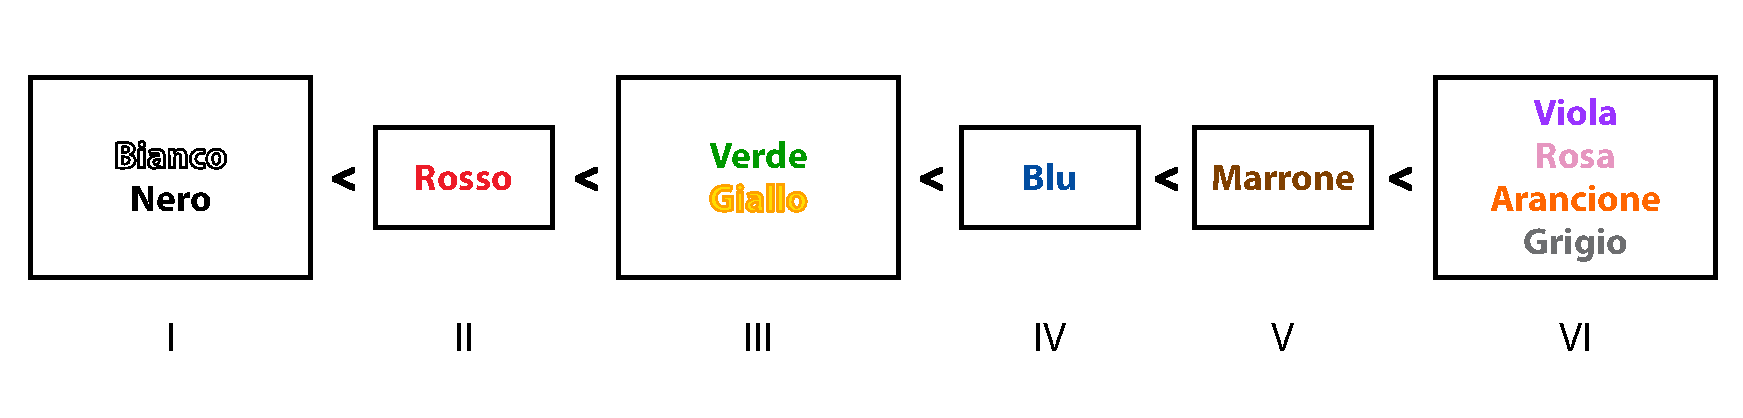
\includegraphics[width=\textwidth]{img/color-category}
  \caption{Le categorie di colori individuate da Berlin e Kay}
  \label{fig:categorie-colori}
\end{figure}

\subsection{I colori nelle lingue}
Alcune lingue, tra cui parecchie della Nuova Guinea, hanno solo due termini fondamentali per i colori, che corrispondono al nero e al bianco o meglio allo scuro e al chiaro. Queste categorie non sono acromatiche, ma pancromatiche. I due colori delle tribù parlanti il Dani, chiamati \emph{mili} e \emph{mola}\index{mili e mola}, includono rispettivamente nero, verde e blu, e bianco rosso e giallo. In questo caso ben tre colori focali sono inclusi nella stessa categoria. Altri termini che si riferiscono ai colori non sono fondamentali perché, ad esempio, sono limitati a oggetti specifici.

Quando un termine include più categorie, immaginiamo ad esempio ``blallo''\index{blallo} come unione delle categorie blu e giallo, il colore focale sarà solo uno di questi due, ma mai un colore derivato da questi. Berlin e Kay propongono l’esempio di ``grue''\index{grue}, come unione di green e blue, il cui colore centrale non è il turchese, ma o il blu o il verde.

Naturalmente vi sono molti più nomi di colori in una lingua come l’italiano: il cremisi, ad esempio, non viene considerato fondamentale perché copre una parte della gamma del rosso, e termini come biondo non vengono considerati perché si applicano solo a certi tipi di oggetti o materiali, analogamente a ciò che avviene in molte società primitive dove i termini che si riferiscono ai colori sono derivati dagli oggetti.

I primi 6 colori sono comunque un sottoinsieme fondamentale che Ewald Hering\index{Hering, Ewald} (1892) identifica come colori primari. Bianco, nero, rosso, verde, giallo e blu, singolarmente o in combinazione formano la base della denotazione dei termini della maggior parte delle lingue di tutto il mondo.

\subsection{Neurofisiologia dei colori}
Il successivo lavoro di Kay e McDaniel (1978) cerca di spiegare i risultati del lavoro di Berlin e Kay usando i lavori di Russell De Valois\index{De Valois, Russell} sulla neurofisiologia dell’apparato visivo dei macachi, simile a quello dell’uomo: nel corpo genicolato della scimmia (la parte del cervello preposta alla visione) De Valois e Jacobs distinguono delle classi di cellule dette \emph{opponenti}: rosso eccitatorio e verde inibitorio e viceversa, giallo eccitatorio e blu inibitorio e viceversa. Insieme a queste cellule si distinguono anche un gruppo di cellule non opponenti, atte a trasmettere la luminosità degli oggetti anziché il loro colore, e comunque un’informazione di tipo acromatico. In termini non tecnici, la visione funziona meglio quando si attiva solo una delle cellule: nel caso della percezione del rosso focale, ad esempio, si attiva la cellula +R –V, mentre le altre non si attivano.

\begin{figure}[hbt]
  \centering
  \includegraphics[width=.5\textwidth]{img/neurofisiologia-colori.png}
  \caption{Schema della neurofisiologia della percezione dei colori. Si passa da uno stimolo tricromatico (RGB) delle cellule della retina ad una percezione basata su sei cellule opponenti}
  \label{fig:neurofisiologia}
\end{figure}

Ipotizzando che le categorie dei colori base siano un prodotto sia della neurofisiologia che della psicologia cognitiva, Key e McDaniel creano un modello di insiemi fuzzy, che combacia con il modello di De Valois e che utilizza unioni ed intersezioni. Secondo questo schema, oltre le 6 categorie primarie, ci sono categorie base derivate (basate sull’intersezione fuzzy) e categorie base composte (basate sull’unione fuzzy). Ad esempio, l’arancione è l’unione di giallo e rosso (derivato), mentre dei colori caldi fanno parte il rosso o il giallo (composto).

\section{Categorizzazione e gerarchia}
Nel testo \emph{How shall a thing be called?} (1956) Roger Brown\index{Brown, Roger} delinea la gerarchia nelle classificazioni. Egli nota che «la dime nella sua tasca non è solo una dime, ma è anche una moneta, un oggetto di metallo, una cosa, e muovendosi nelle sottocategorie è una dime del 1952, una particolare dime del 1952 con un preciso pattern di graffi, scolorature e parti lisce. Un cane non è solo un cane, è anche un boxer, un quadrupede, un animale.» Brown osserva inoltre che di tutti i possibili nomi di qualcosa che sta nella gerarchia di categorie, uno solo tipicamente lo percepiamo come il \emph{vero} nome della cosa. Questi nomi tendono ad essere corti e di uso molto frequente.

Queste categorie base sembrano essere anche associate ad azioni non linguistiche. Ad esempio, alla categoria fiore si associa l’azione dell’odorare, ad una palla si associa l’azione del rimbalzare. Queste azioni sono collegate distintamente a certe categorie e possono funzionare da simbolo per esse. Queste azioni sono strettamente collegate a questo livello della gerarchia: l’azione dell’odorare i fiori, ad esempio, non ci aiuta a distinguere tra le sottocategorie dei fiori.

Il quadro che Brown ci fornisce è che la categorizzazione di base, per i bambini, corrisponde al livello delle azioni distintive delle categorie, per procedere poi verso l’alto con categorie superordinate (come piante e animali) e categorie subordinate (come violette e siamesi). Per queste ultime categorie, infatti, non sembrano esserci azioni distintive. Questo livello di categorizzazione, secondo Brown, deve avere le seguenti proprietà:
\begin{itemize}
  \item è il livello delle azioni distintive;
  \item è il livello che viene appreso per primo e nel quale le cose sono per prime nominate;
  \item è il livello in cui i nomi sono brevi e frequentemente utilizzati;
  \item è un livello di categorizzazione naturale, al contrario al contrario di quelli creati da ``traguardi dell’immaginazione''.
\end{itemize}

La spinta successiva arriva dal lavoro di Berlin\index{Berlin, Brent} le cui ricerche posso essere viste come una risposta alla visione filosofica secondo la quale le categorie della mente corrispondono alle categorie del mondo. Questa dottrina afferma che il mondo consiste largamente di tipi naturali di cose e che il linguaggio naturale contiene nomi (\emph{natural kind terms}) che corrispondono a queste cose. Tipici esempi di cose naturali possono essere cane, mucca, tigre, oro, acqua, ecc.

Per verificare empiricamente questa dottrina filosofica Berlin ha considerato domini nei quali ci sono cose di tipo naturale: il dominio delle piante e degli animali. Il lavoro, essendo egli un antropologo, fu svolto su persone che vivono a stretto contatto con la natura, in particolari abitanti Tzeltal del Chiapas in Messico. Ciò che Berlin e i suoi collaboratori hanno scoperto è che un singolo livello di classificazione, il genere, era psicologicamente basilare per gli Tzeltal in diversi modi. Esempi di piante e animali a livello genere sono quercia, melo, coniglio, procione, ecc. Il primo modo il cui la priorità del genere si è manifestata è stato un semplice lavoro di denominazione. Berlin è semplicemente andato nella foresta assieme a dei nativi e ha chiesto loro di nominare le piante che potevano osservare. I nativi erano in grado di nominarne diversi, ma sempre a livello di generi e mai di specie (anche se studi successivi hanno dimostrato che essi sono in grado di distinguere le specie e di nominarle), tantomeno a livello più generico di forma di vita (albero).

Il livello del genere è, accidentalmente, a metà della gerarchia di classificazione folk (\emph{unique beginner} – piante, animali / \emph{life form} – albero, cespuglio, pesce / \emph{intermediate} – conifera, latifoglia / \emph{genus} – pioppo, faggio, pino, pesce palla, uomo / \emph{species} – pioppo bianco, pioppo tremulo, homo sapiens / \emph{variety} – homo sapiens sapiens).

Studi successivi hanno rivelato che l’utilizzo del genere come livello base non è affatto casuale, ma anzi sembra avere un riscontro psicologico:
\begin{itemize}
  \item le persone nominano le cose più velocemente a questo livello;
  \item le lingue hanno nomi semplici per le cose;
  \item le categorie a questo livello hanno un maggior significato culturale;
  \item le cose vengono ricordate più facilmente;
  \item a questo livello le cose vengono percepite olisticamente, con un singolo gestalt (visione del tutt’uno), mentre per le identificazioni a livelli più bassi dettagli specifici devono essere tirati fuori per distinguere, ad esempio, tra tipi diversi di quercia.
\end{itemize}

\section{Teoria dei prototipi}\index{prototipi, teoria dei}
Gli studi sopra citati sono tutti casi speciali. Eleanor Rosch\index{Rosch, Elanor} è stata la prima a fornire una prospettiva generale a tutti questi problemi. Ha sviluppato quella che viene chiamata  la teoria dei prototipi, stabilizzando la categorizzazione come un sottocampo della psicologia cognitiva. Prima del suo lavoro la teoria classica di classificazione era presa per certa non solo in psicologia, ma anche in linguistica, antropologia, filosofia e altre discipline. I suoi risultati sperimentali rientrano in due categorie: gli effetti prototipo, che estendono la ricerca sui colori di Berlin-Kay e gli effetti di livello base, che generalizzano le osservazioni di Brown e i risultati di Berlin.

Nello studio sulla lingua Dani di Rosch emerge che se la categorizzazione dipendesse solo dalla lingua, come ipotizzato da Whorf\footnote{L'ipotesi di Sapir-Whorf (o Sapir-Whorf Hypothesis, in sigla SWH), altresì conosciuta come \emph{ipotesi della relatività linguistica}, afferma che lo sviluppo cognitivo di ciascun essere umano è influenzato dalla lingua che parla. Nella sua forma più estrema, questa ipotesi assume che il modo di esprimersi determini il modo di pensare.}, allora chi parla Dani avrebbe la stessa difficoltà ad imparare nuovi termini per identificare i colori indipendentemente dal fatto che essi siano focali o meno. Al contrario, i parlanti Dani hanno dimostrato di riuscire a ricordare meglio i colori focali di quelli non focali, mostrando che la rappresentazione in memoria è la stessa di chi parla inglese. I colori focali corrispondo a quello che Rosch identifica come punti di riferimento cognitivi e prototipi.

Rosch ha sviluppato altri esperimenti che hanno fatto emergere asimmetrie (chiamate effetto prototipo) nella classificazione: alcuni membri di categorie sembrano essere più rappresentativi della categoria di altri. Ad esempio, il pettirosso è più rappresentativo della categoria Uccelli della gallina o del pinguino. A sostegno dell’ipotesi Rosch porta l’evidenza sperimentale attraverso interviste dove viene chiesto di valutare:
\begin{description}
  \item[valutazione diretta]esprimere su una scala quanto è buono un membro di una categoria preso come esempio;
  \item[tempo di reazione] ai soggetti viene chiesto di premere un pulsante per indicare vero o falso ad affermazioni tipo ``Un [esempio] è un [nome categoria]''. I tempi di risposta sono minori per gli esempi rappresentativi;
  \item[produzione di esempi] quando viene chiesto di elencare o disegnare esempi dei membri di una categoria, i soggetti disegnano o elencano membri rappresentativi;
  \item[asimmetrie nella similarità di valutazione] gli esempi meno rappresentativi sono spesso considerati essere più simili o rappresentativi dell’opposto. Ad esempio, gli americani considerano gli Stati Uniti altamente rappresentativi di una nazione. I messicani, invece, considerano il Messico più simile agli Stati Uniti che gli Stati Uniti al Messico;
  \item[asimmetria nella generalizzazione] nuove informazioni riguardo i membri delle categorie rappresentative sono generalizzate più facilmente ai membri non rappresentativi (ad esempio, i soggetti credono che sia più facile per le malattie diffondersi dai pettirossi alle anatre su un’isola rispetto al vice versa).
\end{description}

Una delle più interessanti conferme di queste ipotesi arriva dal lavoro di Barsalou (1983). Egli studiò quello che chiama \emph{categorie ad hoc}\index{categorie ad hoc}, ovvero categorie che non sono convenzionali o fisse, ma piuttosto create al volo per qualche intento immediato. Queste categorie vanno create sulla base del modello cognitivo riguardante la materia presa in considerazione. Esempi di queste categorie sono \emph{le cose ce si prendono da casa durante un incendio}, \emph{i regali di compleanno}, \emph{cosa fare nel week end}. Barsalou osserva che queste categorie hanno una struttura prototipale che non esiste in anticipo, perché la categoria non esiste o non è convenzionale. In questi casi la natura della categoria viene determinata dall’obiettivo e la struttura di questo obiettivo è funzione del proprio modello cognitivo.

Un ultimo concetto della teoria di Rosch riguarda le proprietà. Alcuni attributi, come ``posto'' per l’oggetto ``sedia'', non hanno senso se non in relazione alla conoscenza dell’oggetto come sedia. Attributi come ``grande'' hanno senso in relazione alla categorizzazione superordinata, ad esempio ``grande piano'' ha senso rispetto alla categoria delle ``forniture'', ma non rispetto agli ``edifici''. Attributi come ``ci puoi mangiare sopra'' hanno senso per l’oggetto ``tavolo'' nella misura in cui abbiamo conoscenza sulle abitudini dell’uomo. Per questo la nozione di proprietà non è qualcosa oggettivamente nel mondo indipendentemente da qualsiasi esistenza, è piuttosto qualcosa che si riferisce ad una proprietà di interazione, il risultato della nostra interazione come parte dell’ambiente fisico e culturale.

\section{Gestalt}\index{gestalt}
La \emph{gestalt} è una scuola psicologica, chiamata anche psicologia della forma (e in tedesco \emph{Gestaltpsychologie}), nata in Germania negli anni immediatamente precedenti la Prima Guerra Mondiale, i cui massimi esponenti furono M. Wertheimer, K. Koffka e W. Köhler. La concezione fondamentale alla base della gestalt è che nella nostra percezione del mondo esterno noi non cogliamo delle semplici somme di stimoli, i quali si uniscono a dare gli oggetti, ma percepiamo delle forme, che sono qualcosa di più e di diverso della semplice somma degli stimoli che la compongono. Tale teoria si opponeva polemicamente a quanto sostenevano gli psicologi associazionisti ed elementaristi i quali concepivano invece il processo percettivo come una semplice opera di sommazione degli stimoli e vedevano il lavoro dello psicologo soprattutto come un'opera di analisi del percepito, in cui era importante separare il momento della “sensazione” da quello della vera e propria “percezione”. Per gli psicologi della forma, invece, tale analisi non era possibile, essendo le forme stesse le minime unità d'analisi, ulteriormente inscindibili; essi pensavano inoltre che le forme si costituissero sulla base di certe leggi percettive sostanzialmente innate, legate alla dinamica del sistema nervoso, mentre per gli associazionisti i legami fra le sensazioni elementari si costituivano sulla base dell'esperienza passata dell'individuo. La nascita della Gestalt si ebbe con un famoso esperimento di Wertheimer, del 1911, sul movimento apparente o stroboscopico: il ``fenomeno phi''.

Il focus della teoria della gestalt è l’idea del raggruppamento. I fattori primari che lo determinano sono:
\begin{description}
  \item[prossimità] gli elementi tendono ad essere raggruppati in accordo con la loro prossimità;
  \item[similarità] oggetti simili tendono ad essere raggruppati;
  \item[completezza] gli oggetti vengono raggruppati se tendono a completare una certa entità;
  \item[semplicità] gli oggetti vengono raggruppati secondo semplici figure, utilizzando simmetrie, regolarità e levigatezza.
\end{description}